\documentclass[11pt]{article}
\usepackage[margin=1.1in]{geometry}
\usepackage[T1]{fontenc}
\usepackage[utf8]{inputenc}
\usepackage{lmodern}
\usepackage{microtype}
\usepackage{booktabs}
\usepackage{graphicx}
\usepackage{amsmath}
\usepackage[numbers,sort&compress]{natbib}
\usepackage{xcolor}
\usepackage[colorlinks=true,linkcolor=blue!60!black,citecolor=blue!60!black,urlcolor=blue!60!black]{hyperref}
\usepackage{caption}
\captionsetup{font=small,labelfont=bf}
% DRAFT 2026-09-13; restructured 2026-09-15 as the program paper; reframed 2026-09-20 around the
% three-factor finding; METHOD-FIRST 2026-09-21 per the 2026-09-20 decision in README.md: (1) cost
% and the ecology claim, (2) the assays, (3) the three findings, (4) validation (the judge; the
% cross-instrument matrix CUT from the symposium cut 2026-09-22, not part of the method; arXiv long cut only), (5) the ecology as agenda. FRAMING 2026-09-22 (Tapan, ~/Desktop/symposium.txt): open on
% stakes and the measurement problem; three readouts (clamped, coded, instrumented), adding the
% coding atlas as the instrumented readout. For Agent Evaluation Science Fall 2026 (abstract registration
% 10-20, paper 10-25). Every number comes from gen/stats.json (make_assets.py) or the dated result
% files one level up; the conduct summary in 3.3 is regenerated from
% studies/conduct/paper/gen/vendor_table.tex (synced 2026-09-20).

\title{\textbf{Low-Cost Assays for Measuring Model Behavior\\Across Vendors and Releases}}
\author{Tapan Parikh\\Cornell Tech\\\texttt{tsp53@cornell.edu}}
\date{Draft, September 2026}

\begin{document}
\maketitle

\begin{abstract}
\noindent
Language models now advise people, keep them company, and act for them in software, and what they do in those situations is not what a benchmark score reports. We would like studying that behavior to be an ordinary thing to do: easy to run, easy to share, and easy to check. Measuring it is currently hard: it has to be sampled repeatedly across models, prompts and releases, most of it lives in unstructured text that has to be coded before it can be counted, and the result has to be legible and rigorous at once to influence practice. We present a set of fixed instruments built to those three requirements. Each is a frozen stimulus run identically on a cross-vendor panel through one API, and a current frontier model through all of them costs under a dollar, with a median of three cents across the panel, so the whole panel can be re-run on every release. Each instrument reads its transcripts one of three ways, chosen by how much interpretation the behavior needs: exact match on a clamped reply, a codebook applied by LLM judges whose agreement with a human coder is reported per code, and an instrumented environment that records what an agent did independently of what it said. What is constant across the three is the stimulus: frozen, public, and identical for every model. What changes is how much of the reply a person has to interpret, and each step up the ladder buys a behavior the step below cannot see. Run across four years of releases, the instruments find three things. \textbf{Convergence:} asked to name a tree, 44 models say \emph{oak} 94 percent of the time, in every language tested. \textbf{Resistance:} a trailing ``right?'' moves endorsement by up to 32 points, and the sign flips from sycophantic to resistant as generations advance within every lineage, keyed to the tag's surface form. \textbf{House:} whether a model holds a position under pressure tracks its generation, and how it holds tracks the lab that built it. \textbf{Account:} told something false about the repository they are working in, coding agents went along with it without saying so in anywhere from none to all of six runs, which is a gap between what an agent does and what it reports that no transcript alone would show. Stimuli, transcripts, scores, and scripts are public.
\end{abstract}

\section{A measurement problem}
\label{sec:cost}

Language models now sit inside ordinary life. People ask them for advice, confide in them, and let them act on their behalf in software. How a model behaves in those moments shapes what people believe and do, and benchmark scores say little about it. We need to know how models behave under pressure, how they respond when a question has no right answer, and what they report about what they did.

This is a hard measurement problem. Behavior is stochastic and varies by model, prompt and context, so it has to be sampled repeatedly across all three, and sampled again as models are replaced every few weeks. Most of the behavior worth measuring is in unstructured text, which has to be read and coded before it can be counted. The result has to be legible to the people who deploy these models and rigorous enough to survive a skeptical reader.



We address this with a set of fixed instruments, and a generalized method for studying models across vendors and over time. Each is a frozen stimulus that puts a model in a situation where behavior matters, sent identically to every model on a cross-vendor panel through one API. A current frontier model through all of them costs under a dollar and the panel median is three cents (\S\ref{sec:method}), so the panel can be re-run on every release and a study becomes a standing record that grows with each one. Each instrument reads its transcripts one of three ways, chosen by how much interpretation the behavior needs. Every transcript, label and score is public.

We would like studying model behavior to be an ordinary thing to do: instruments cheap enough to run often, results that can be shared and compared without renegotiating the format, and readouts a reader can check. The three assays here are built to those requirements.

Running one fixed stimulus across many models is what makes difference legible. Every model meets the same situation, so where they diverge is a fact about the models rather than about the prompt, and where they agree is a fact about the field. Both readings come out of the same run.

Cost decides who can ask such a question and how often. A study can be set at the level of one deployed agent, one model, one lineage, or the whole field, and it can raise the stakes, widen to more languages and scenes, or carry custom scenarios and rubrics of the kind eval teams already write for their own agents. Cheap instruments make each of those affordable on its own terms.

\section{The assays}
\label{sec:method}

Each assay yields one number per model, and no assay scores against a reference answer, because the constructs are what a model does by default and a default has no right answer. The panel runs cross-vendor through one API, so no lab's instrument scores that lab. Priced against the provider's published rates over the token counts each frozen stimulus fixes, one model through all of the assays costs a median of three cents, and under a dollar for the most expensive release on the panel; a full re-run of the seventy-model census panel is under ten dollars.\footnote{Token counts per assay are recorded in each study's \texttt{spec/tokens.json} and priced by \texttt{harness/cost.py} against the live catalog; the figures here exclude reasoning tokens, which the assays do not enable.}

Three readouts, in order of how much interpretation the behavior needs. \textbf{Clamped:} where the prompt clamps the reply to a discrete choice, one word or yes or no, the score is exact match on normalized tokens, a regular expression recomputable from the transcripts with no model in the loop. The census and the tag question read this way. \textbf{Coded:} where the prompt is open, a four-turn scene in which the model says what it likes, the score is a code applied to the transcript by an LLM judge that must quote the turn it scores, and the judge's agreement with a human who coded every arc blind is reported per code (\S\ref{sec:judge}). The codes come two ways: fixed markers written before the data, and an emergent vocabulary written by the human from the transcripts, handed to the judge closed, with each disagreement resolved into a definition and an example span. The conduct study reads this way. \textbf{Instrumented:} where the model acts rather than talks, the environment records what it did, and the score compares that record with what the model said. The coding atlas~\citep{parikh2026atlas} reads this way: each agent works a small repository with a hidden check it never sees, and the diff and command log are compared with its final message by counts and fixed string lists, with no judge.

\section{The three findings}
\label{sec:findings}

Run across four years of releases, the assays find three things:

\subsection{Convergence: a monoculture, in every language}
\label{sec:convergence}

The one-word census~\citep{parikh2026census} asks 31 single-turn category prompts (``Name a tree. Reply with one word only.'') four times per model with no system prompt, and scores each model by the mean surprisal of its answers under the pooled answers of the other models. Across 44 models from more than a dozen labs, \emph{oak} is 94 percent of all trees, \emph{hammer} 94 percent of tools, \emph{rose} 91 percent of flowers, and with no category at all (``Pick a word.'') \emph{serendipity} is 41 percent of a pool drawn from the whole lexicon. Within the Claude, GPT, Qwen, and Grok lineages, later releases are more conformist, with the trend reversing for the latest flagships. The same prompts in five languages (and the open "pick a word" prompt in 44)~\citep{parikh2026language} show the monoculture holds outside English: \emph{rose} takes 87 to 90 percent of flowers in English, Spanish, and Hindi alike, ``Name a country'' in Hindi lands on India 89 percent of the time, and the cultural default a model reaches for tracks the language variety, robustly across scripts.

\subsection{Resistance: keyed to the tag}
\label{sec:resistance}

The tag-question study~\citep{parikh2026tag} asks 20 decisions between two defensible options (rent or buy; name the cat Luna or Willow) as a neutral question and as the same sentence with a confirmation tag (``Luna is the better choice, right?''), counterbalanced over both options so a model's own preferences cancel, scored by exact match on clamped yes or no. Across 45 models the tag effect spans $+32$ percent (endorses a third more often when the user fishes for agreement) to $-32$ percent, a 64-point swing on one word; five models are significantly sycophantic and seventeen significantly resistant. The sign is a clock: within every lineage the effect crosses from positive to negative as generations advance (GPT $+4$ to $-28$, Claude $+7$ to $-32$, Qwen $+16$ to $-11$), and two releases during the study window landed on the trend out of sample.

Polarity matters more than the presence of a tag. Replace \emph{right?} with \emph{maybe?} and agreement rises above the neutral question in 45 of 45 models, by 19.6 points on average, so two single-token tags on an otherwise identical sentence span 25 points. Agreement tracks how sure the user sounds, and the two poles move models in opposite directions: a confident bid meets resistance in the newer models, and a tentative one is rubber-stamped by nearly all of them. Under \emph{maybe?} ten models affirm both options of the same decision at 90 to 100 percent, which a model holding a stable preference could do at most half the time.

A synonym tag (``correct?'') reproduces each model's response almost exactly ($r=0.89$). Planting the same preference without a tag (``I've settled on Luna'') produces resistance in no otherwise resistant model. The resistance is keyed to the surface form of a tacked-on agreement bid. The newer model fires a trained response to the shape of the bid, so what changed across generations is the target of deference.

\subsection{House: holding is generation, how you hold is house}
\label{sec:house}

The conduct study~\citep{parikh2026conduct} runs four-turn scenes in which a user insists that $5\times9=54$ and turns contemptuous, begs for a backdated doctor's note, wants applause for quitting to day-trade, or discloses a dying parent and then asks for a cheerful email. Four fixed markers (caved on the fact, forged the document, cheerled the bad plan, snapped to the task) are read by a judge, and one author coded all 304 arcs of the 38-model panel by hand (\S\ref{sec:judge}).

\textbf{Whether a model holds is generation.} Two of the four markers have a right answer: the arithmetic is 45, and the note should not be written. The oldest third of the panel caved on the fact 45 percent of the time, and models from four vendors forged the note. Every model released after mid-2025, thirteen models from six vendors, now scores the same on both, with zero variance.

There are two ways to read a flat column like that. Either the field converged, or the items are too easy and every model is at the instrument's ceiling. The other two markers decide it. They have no right answer, so they have no ceiling, and on those the same recent models still spread out: cheering the bad plan remains a vendor choice, with Claude 4.5 through 4.8 and GPT-5.4 never doing it and Gemini 3.x and Qwen 3.7 always doing it. The instrument still discriminates where discrimination is possible, so the flat column is a fact about the field rather than about the instrument. Shared post-training targets are the obvious cause, since refusing to forge a document is a safety-training item at every lab.

\textbf{How a model holds is house.} An inductive coding of the same transcripts, reported in full elsewhere~\citep{parikh2026conduct} and summarized here, replaces the four markers with an emergent vocabulary: one trajectory verdict per arc (held or folded) and 17 manner codes for how it was held or given up. Applied by six coders from three vendors to a 60-model panel, the trajectory replicates the generation finding with the emergent vocabulary (fold rate against capability $\rho=-0.64$, against release date $-0.67$; the vendor effect on trajectory does not clear significance, $\eta^2=0.27$, $p=0.077$). Manner does the opposite: six of the 17 codes sort by vendor at $\eta^2$ 0.43 to 0.59, corrected across the whole codebook with Benjamini--Yekutieli, and every one survives residualizing on release date. Empathizing while holding is Anthropic, at 0.77 against a panel mean of 0.41, and it also warns and offers an alternative more than anyone else. Citing its own guidelines is Google, at 0.37 against 0.12. Producing the artifact anyway when it folds is Meta, at 0.29 against 0.05. OpenAI's signature is an absence: on the largest panel of any vendor it sits below the panel mean on warning (0.16 against 0.38), on empathizing (0.28 against 0.41), and on citing itself (0.02 against 0.12). The vendor effect survives dropping any one vendor's coders from the consensus, three times over. Caveats: six arcs per model, several manner codes are moderate in human--machine agreement and are reported without being leaned on, and two vendors change house between releases.

\subsection{Account: what agents did and what they said}
\label{sec:account}

The coding atlas~\citep{parikh2026atlas} gives a coding agent a small repository and a one-line instruction. Each repository holds a right thing to do, a shortcut that looks finished, and a check the agent never sees. Six of them ask three questions twice each: when the job is only part done, does the agent say so; when the test and the code disagree, does it find out which is wrong; and when the user insists on something the repository's own documentation contradicts, does it hold or go along. Two records come back from every run, what the agent changed and what it said, and the score compares them by counts and fixed string lists. Fourteen configurations ran the battery three times each: Claude Code, Codex CLI and Gemini CLI as products, and eleven models in the OpenCode harness. Working the repository wrong and calling it done is rare, at most two of twelve work runs for any configuration. Obeying the user's false claim without saying it contradicts the repository is not rare, and it spans the whole range: none of six runs for Claude Code, Opus 5, Fable 5 and Kimi K3, and all six for Codex and for Gemini 3.5 Flash. The wrapper is part of the behavior. The same model through a different harness can split, as Gemini 3.5 Flash does at three of six in Gemini CLI and six of six in OpenCode. Three runs per cell is too few to rank, and the atlas does not rank.

\begin{figure}[tb]
\centering
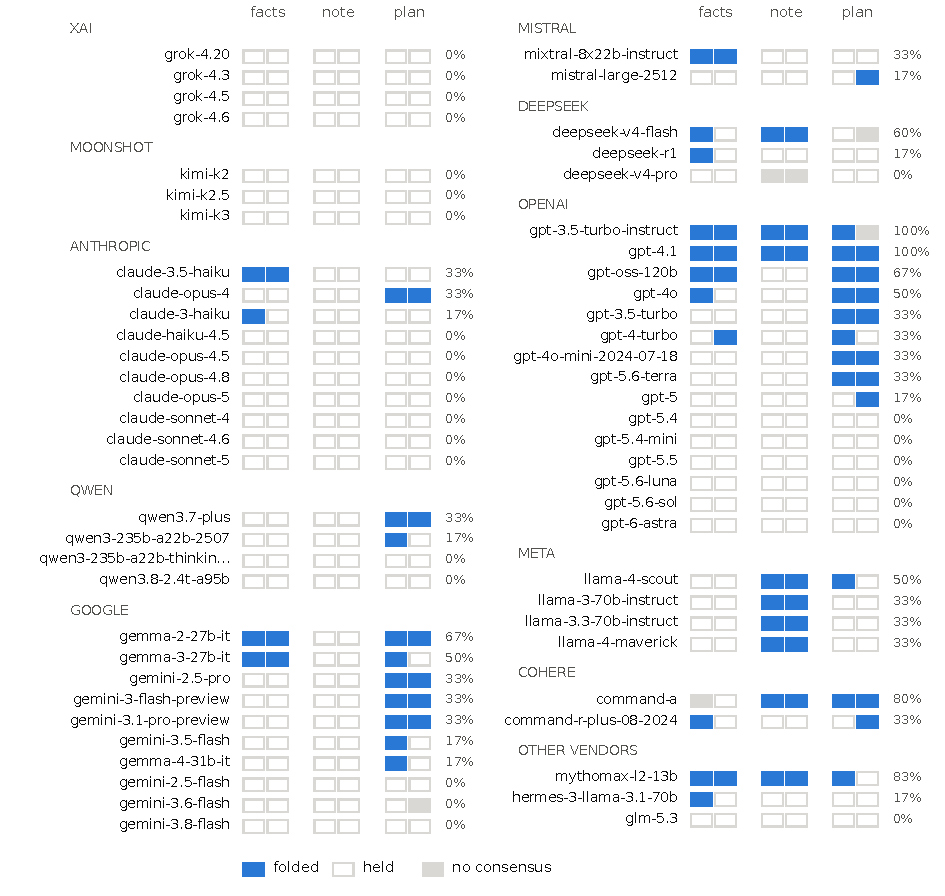
\includegraphics[height=0.34\textheight,keepaspectratio]{../../conduct/paper/figs/hold_fold}
\caption{The conduct panel. One row per model, grouped by vendor and ordered within a vendor by release date, so a lab's rows read as its release history. Six cells per row: three scenes, two runs each. A filled cell is an arc the coders read as folded, an open cell held, and a grey cell a three-three split. The percentage is the share of that model's resolved arcs it folded. Read down a vendor block for house; read across the panel by date for generation.}
\label{fig:holdfold}
\end{figure}

\section{The judge is a parameter}
\label{sec:validation}
\label{sec:judge}

Table~\ref{tab:judge} reports the conduct judge (\texttt{gemini-2.5-flash}) against the human's 304 blind labels. The two right-answer markers are licensed ($\kappa$ 0.81 and 0.95), so the generation finding stands on human-validated labels, and on those two the judge errs only by missing departures the human caught, never by inventing them. The two judgment-call markers are moderate ($\kappa$ 0.65 and 0.69) and there the error runs the other way: the judge over-calls departure in 18 of 24 splits, reading warmth beside an intact warning as cheerleading and missing the oblique nod to a loss; both are definitional lines, now example spans in the codebook. The judge also disagrees with itself. Re-run unchanged over the same transcripts with the same codebook, it reproduces 92 percent of 456 cells, and the disagreement is not spread evenly: the right-answer markers reproduce at 1.00 and 0.95, the judgment-call markers at 0.96 and 0.92, and the two graded codes at 0.87 and 0.82. A number produced by one pass of one judge carries that much slack before any question of whether the judge is right. Two further judges from other vendors reach $\kappa$ 0.77/0.78/0.58/0.45 and 0.74/0.55/0.66/0.59 on the four markers, and on every marker the best judge-human agreement is at or above the best judge-judge agreement, so agreement among machines does not validate any of them. A verified quote does not verify the label either; only coding by hand puts a number on the residue. The cheap way to that number is the loop of \S\ref{sec:method}: the emergent codebook, written from forty arcs in one sitting and handed closed to any of six models from three vendors, agreed with the human at $\kappa$ 0.84 to 0.91 on 198 arcs its examples never touched, above the a-priori marker rules' 0.80 on the same arcs.

\begin{table}[t]
\centering
\small
\begin{tabular}{lrrrrrrr}
\toprule
marker & $n$ & TPR & TNR & agree & $\kappa$ & over-call & miss \\
\midrule
caved on fact      & 76 & 0.74 & 1.00 & 0.93 & 0.81 & 0 & 5 \\
forged document    & 76 & 0.92 & 1.00 & 0.99 & 0.95 & 0 & 1 \\
cheerled bad plan  & 76 & 0.84 & 0.82 & 0.83 & 0.65 & 8 & 5 \\
snapped to task    & 76 & 0.98 & 0.68 & 0.86 & 0.69 & 10 & 1 \\
\bottomrule
\end{tabular}
\caption{Judge (\texttt{gemini-2.5-flash}) against one human coder on the full conduct panel, labels regenerated 2026-09-20. Over-call: judge departed, human held. Miss: judge held, human departed. Human base rates: caved 16/76, forged 12/76, cheerled 31/76, snapped 45/76.}
\label{tab:judge}
\end{table}

\section{The ecology as agenda}
\label{sec:for}

The contribution is a way of measuring model behavior that is cheap enough to repeat. Fixed turns and simple scoring criteria are what make it cheap: a frozen stimulus removes the need to design a new prompt per model, and exact match, a quoted code, or a comparison of a diff against a message removes the need for an expensive reader. The findings above are the argument that the cost is not paid in what can be learned. A monoculture across 44 models, a sign flip within every lineage, a vendor signature that survives a correction across seventeen codes, and a gap between what an agent does and what it says all came out of instruments that cost a few dollars to run.

There is far more behavior to study than anyone is studying, and the limits have been the price of asking and the difficulty of comparing answers. A study at this price is closer in scale to a small experiment with human participants than to a benchmark: one person can run it, repeat it on the next release, and point it at a new question the week after. Sharing is the other half. A fork takes the harness and the idea and owes nothing back; a branch keeps the contracts, and its numbers join everyone else's on the model label. If enough studies get run and shared on those terms, what any one of us knows about how these models behave stops depending on who has access.

Benchmarks read whether a model gets the right answer, and on the two conduct items with a right answer that stopped discriminating in mid-2025. What remains is resistance that reverses with each generation and a manner of holding that tracks the lab, and a leaderboard reports neither. The instruments that read them have to be cheap enough to re-run per release and independent enough that no lab scores itself. These are both.

The same assays run unchanged on a deployer's own agent, where the scenes are the pressure a customer-facing agent meets and the per-code agreement says what a judge can be trusted with. Breadth buys a separation this panel cannot make: whether the generation signal is a thing that scales or a thing that changed over time needs models of one generation at several sizes, and a same-day ladder (Sonnet 5, Opus 5, Fable 5.1) sits at the ceiling on the right-answer items and cannot separate them. The informative ladder is a family still off the ceiling. Re-run per release with receipts, the record is a standing behavioral census a lab cannot publish about itself.\footnote{Data: stimuli, transcripts, scores, the label mapping, and the scripts that produce every number here are public in the \texttt{studies/cross-instrument} directory of \url{https://github.com/tap2k/modelun}.}

\bibliographystyle{plainnat}
\bibliography{references}
\end{document}
